\subsection{Grobkonzept 1} \label{subsec:grobkonzept1}
\definecolor{dpink}{HTML}{FF13F8}
\definecolor{hpink}{HTML}{FF98FC}
\definecolor{hgruen}{HTML}{9EFFA9}
\definecolor{hblau}{HTML}{51D1FF}
\definecolor{dblau}{HTML}{008BBD}
\definecolor{hgelb}{HTML}{FFFC9E}
\definecolor{dgelb}{HTML}{FFCC67}
\definecolor{dgruen}{HTML}{00AC14}

\newcommand{\titleCell}[2]{\multicolumn{3}{c}{\cellcolor{#1}#2}}
\newcommand{\cC}[1]{\cellcolor{#1}}

%\newcommand{\HY}{\hyphenpenalty = 25\exhyphenpenalty = 25}
\begin{table}[H]
\small
\begin{tabular}{>{\HY\RaggedRight}p{3cm} >{\HY\RaggedRight}p{3.6cm} >{\HY\RaggedRight}p{6.9cm} r}
\hline
\textbf{Bestandteil}&\textbf{Typ}&\textbf{Funktion}&\textbf{Anz.}\\
\hline

\rowcolor{hellgrau}
\multicolumn{4}{l}{\textbf{Stromerzeugung}}\T\\
Wasserrad& &Umwandlung in Rotationsenergie&43\\
Generator&AC&Umwandlung in elektrische Energie&43\\
Gleichrichter&AC/DC Wandler&Wechselstrom zu Gleichstrom&43\\
DC/DC Konverter&&Regelt die Spannung für den DC Bus&43\\
Wechselrichter&&Umwandlung DC in AC (230V) &1\B\\

\rowcolor{hellgrau}
\multicolumn{4}{l}{\textbf{Kontrollsystem}}\T\\
PC&&Anlagesteuerung&1\\
SPS&Beckhof&Analoge und Digitale Ein- und Ausgänge&1\B\\

\rowcolor{hellgrau}
\multicolumn{4}{l}{\textbf{Abwassertechnik}}\T\\
Bypass&Absperrklappe&Umleitung für Wartungsarbeiten und Störungen an den Wasserräder&43\B\\


\hline
\end{tabular}
\caption{Bestandteilliste Grobkonzept 1}\label{tab:BLGrobkonzept1}
\end{table}

Im Grobkonzept 1 sollen 43 Wasserräder direkt in die Fallleitung eingebaut werden. Mit jeweils einem Generator pro Wasserrad wird Strom erzeugt. Damit der Strom der einzelnen Wasserräder zusammengeführt werden kann, muss der Wechselstrom zuerst in Gleichstrom umgewandelt werden. Dieser wird auf einen DC-DC Konverter gelegt. Anschliessend wird der Gleichstrom mit einem Wechselrichter auf die Netz-Spannung umgewandelt. Ein Kontrollsystem steuert die Anlage, überwacht die Energiegewinnung und schreitet bei Störungen ein. In unserem Hochhausmodell (Park Avenue 432) wird immer nach zwei Etagen ein Wasserrad eingebaut, um die maximale Leistung herausholen zu können. 
\newpage
\begin{wrapfigure}{r}{0.5\textwidth}
  \begin{center}
    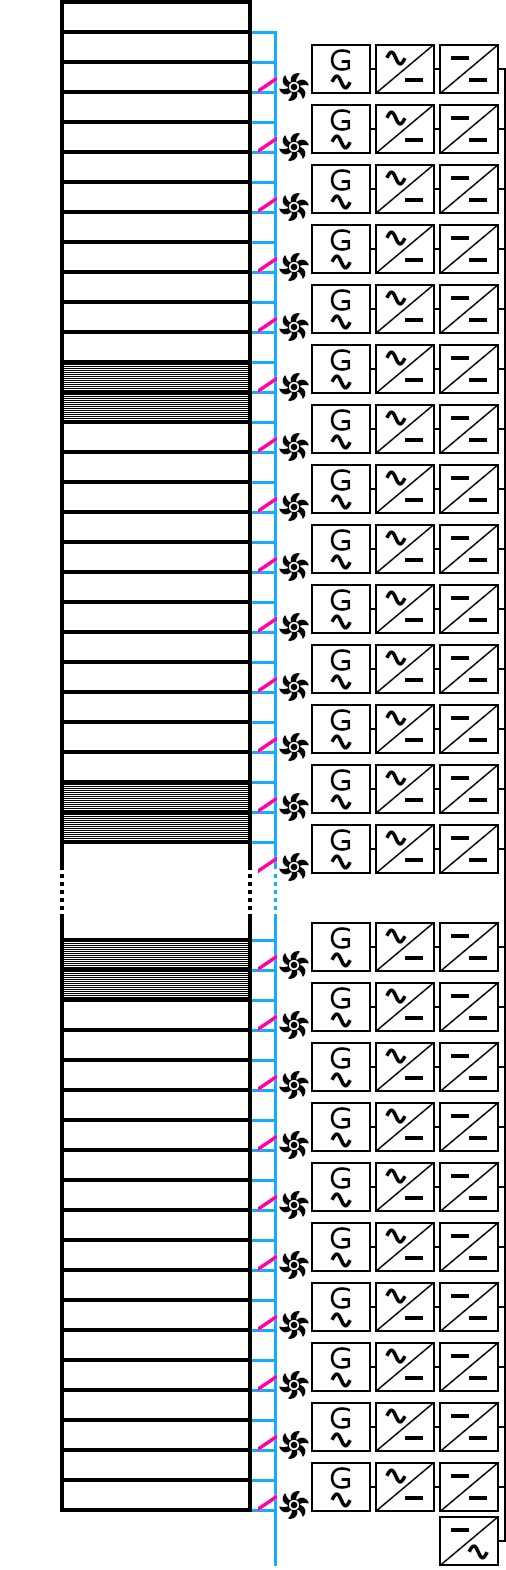
\includegraphics[width=0.48\textwidth]{grobkonzept1}
  \end{center}
  \caption{Schema Grobkonzept 1}
\end{wrapfigure}
\bigskip

\textbf{Vorteile:}								\newline
+	platzsparend									\newline
+	keine zusätzlichen Leitungen
	
\textbf{Nachteile:}								\newline
-	Luftwiderstand								\newline
- 	defektanfällig								\newline
-	AC-DC-AC Umwandlung							\newline
\WFclear
\newpage

